\section{Operations with ellipsoids}
\todo[inline]{Renamed all variables according to the coding policy}
In the {\it Ellipsoidal Toolbox} we define a new class {\tt ellipsoid} inside
the MATLAB programming environment. The following three commands
define the same ellipsoid $\EE(q,Q)$, with $q\in{\bf R}^n$ and
\todo[inline]{Updated all methods' calls according to the the new OOP}
$Q\in{\bf R}^{n\times n}$ being symmetric positive semidefinite:
\verbmcodef[Definition of the ellipsoid]{mcodesnippets/s_chapter05_section01_snippet01.m}
For the {\tt ellipsoid} class we overload the following functions and operators:
\begin{itemize}
\item {\tt isempty(ellObj)} - checks if $\EE(q,Q)$ is an empty ellipsoid.
\item {\tt display(ellObj)} - displays the details of ellipsoid $\EE(q,Q)$, namely,
its center $q$ and the shape matrix $Q$.
\item {\tt plot(ellObj)} - plots ellipsoid $\EE(q,Q)$ if its dimension is not greater
than 3.
\item {\tt firstEllObj == secEllObj} - checks if ellipsoids $\EE(q_1,Q_1)$ and
$\EE(q_2,Q_2)$ are equal.
\item {\tt firstEllObj \~{ }= secEllObj} - checks if ellipsoids $\EE(q_1,Q_1)$ and
$\EE(q_2,Q_2)$ are not equal.
\item {\tt [ , ]} - concatenates the ellipsoids into the horizontal array, e.g.
{\tt ellVec = [firstEllObj secEllObj thirdEllObj]}.
\item {\tt [ ; ]} - concatenates the ellipsoids into the vertical array, e.g.
{\tt ellMat = [firstEllObj secEllObj; thirdEllObj fourthEllObj]} defines $2\times 2$ array of ellipsoids.
\item {\tt firstEllObj >= secEllObj} - checks if the ellipsoid {\tt firstEllObj} is bigger than
the ellipsoid {\tt secEllObj}, or equivalently $\EE(0,Q_1)\subseteq\EE(0,Q_2)$.
\item {\tt firstEllObj <= secEllObj} - checks if $\EE(0,Q_2)\subseteq\EE(0,Q_1)$.
\item {\tt -ellObj} - defines ellipsoid $\EE(-q,Q)$.
\item {\tt ellObj + bScal} - defines ellipsoid $\EE(q+b,Q)$.
\item {\tt ellObj - bScal} - defines ellipsoid $\EE(q-b,Q)$.
\item {\tt aMat * ellObj} - defines ellipsoid $\EE(q,AQA^T)$.
\item {\tt ellObj.inv()} - inverts the shape matrix of the ellipsoid: $\EE(q,Q^{-1})$.
\end{itemize}
All the listed operations can be applied to a single ellipsoid as well as to
a two-dimensional array of ellipsoids.
For example,
\verbmcodef[Examples of the operation]{mcodesnippets/s_chapter05_section01_snippet02.m}
To access individual elements of the array, the usual MATLAB subindexing
is used:
\verbmcodef[Access to individual elements]{mcodesnippets/s_chapter05_section01_snippet03.m}
Sometimes it may be useful to modify the shape of the ellipsoid without
affecting its center. Say, we would like to bloat or squeeze the ellipsoid:
\verbmcodef[Modification of the ellipsoid's shape]{mcodesnippets/s_chapter05_section01_snippet04.m}
Since function {\tt shape} does not change the center of the ellipsoid,
it only accepts scalars or square matrices as its second input parameter.
Several functions  access the internal data of
the ellipsoid object:
\verbmcodef[Get the center and the shape matrix of ellipsoid]{mcodesnippets/s_chapter05_section01_snippet05.m}
\verbmcodef[Check if given ellipsoids are degenerate]{mcodesnippets/s_chapter05_section01_snippet06.m}
\verbmcodef[Get space dimensions and ranks of the shape matrices]{mcodesnippets/s_chapter05_section01_snippet07.m}
One way to check if two ellipsoids intersect, is to compute
the distance between them:
\verbmcodef[Computation of the distance between ellipsoids]{mcodesnippets/s_chapter05_section01_snippet08.m}
This result indicates that the ellipsoid {\tt thirdEllObj} does not intersect with
the ellipsoid {\tt ellMat(2, 2)}, with all the other ellipsoids in {\tt ellMat}
it has nonempty intersection. If the intersection of the two ellipsoids is
nonempty, it can be approximated by ellipsoids from the outside as well as
from the inside:
\verbmcodef[Approximation of the ellipsoids' intersection]{mcodesnippets/s_chapter05_section01_snippet09.m}
It can be checked that resulting ellipsoid {\tt externalEllObj} contains the given
intersection, whereas {\tt internalEllObj} is contained in this intersection:
\verbmcodef[Check if the ellipsoid contains the intersection]{mcodesnippets/s_chapter05_section01_snippet10.m}
\verbmcodef[Check if the internal approximation is contained in the intersection]{mcodesnippets/s_chapter05_section01_snippet11.m}
Function {\tt isinside} in general checks if the intersection of ellipsoids
in the given array contains the union or intersection of ellipsoids or
polytopes.

It is also possible to solve the feasibility problem, that is, to check
if the intersection of more than two ellipsoids is empty:
\verbmcodef[Check if the intersection of more than two ellipsoids is empty]{mcodesnippets/s_chapter05_section01_snippet12.m}
In this particular example the result $-1$ indicates that the intersection
of ellipsoids in {\tt ellMat} is empty.
Function {\tt intersect} in general checks if an ellipsoid,
hyperplane or polytope intersects the union or the intersection
of ellipsoids in the given array:
\verbmcodef[Check if ellipsoid intersects the ellipsoids' intersection]{mcodesnippets/s_chapter05_section01_snippet13.m}
\verbmcodef[Check if ellipsoid intersects the ellipsoids' union]{mcodesnippets/s_chapter05_section01_snippet14.m}
For the ellipsoids in ${\bf R}$, ${\bf R}^2$ and ${\bf R}^3$ the geometric
sum can be computed explicitely and plotted:
\verbmcodef[Compute and plot the geometric sum of ellipsoids]{mcodesnippets/s_chapter05_section01_snippet15.m}
If the dimension of the space in which the ellipsoids are defined exceeds $3$,
an error is returned. The result of the geometric sum operation is
not generally an ellipsoid, but it can be approximated by families
of external and internal ellipsoids parametrized by the direction vector:
\verbmcodef[Approximation of the geometric sum's result]{mcodesnippets/s_chapter05_section01_snippet16.m}

Functions {\tt minksum\_ea} and {\tt minksum\_ia} work for ellipsoids of
arbitrary dimension. They should be used for general computations
whereas {\tt minksum} is there merely for visualization purposes.

If the geometric difference of two ellipsoids is not an empty set, it can
be computed explicitely and plotted for ellipsoids in ${\bf R}$,
${\bf R}^2$ and ${\bf R}^3$:
\verbmcodef[Geometric difference]{mcodesnippets/s_chapter05_section01_snippet17.m}
Similar to {\tt minksum}, {\tt minkdiff} is there for visualization
purpose. It works only for dimensions $1$, $2$ and $3$, and for higher
dimensions it returns an error. For arbitrary dimensions, the geometric
difference can be approximated by  families of external and internal
ellipsoids parametrized by the direction vector, provided this direction
is not bad:
\verbmcodef[Approximation of the geometric difference's result]{mcodesnippets/s_chapter05_section01_snippet18.m}
Operation 'difference-sum' described in section 2.2.4 is implemented in
functions {\tt minkmp}, {\tt minkmp\_ea}, {\tt minkmp\_ia}, the first one of
which is used for visualization and works for dimensions not higher than $3$,
whereas the last two can deal with ellipsoids of arbitrary dimension.
\verbmcodef[Implementation of an operation 'difference-sum']{mcodesnippets/s_chapter05_section01_snippet19.m}
Similarly, operation 'sum-difference' described in section 2.2.5
is implemented in
functions {\tt minkpm}, {\tt minkpm\_ea}, {\tt minkpm\_ia}, the first one of
which is used for visualization and works for dimensions not higher than $3$,
whereas the last two can deal with ellipsoids of arbitrary dimension.
\verbmcodef[Implementation of an operation 'sum-difference']{mcodesnippets/s_chapter05_section01_snippet20.m}
\section{Operations with hyperplanes}
The class {\tt hyperplane} of the {\it Ellipsoidal Toolbox} is used
to describe hyperplanes and halfspaces. The following two commands
define one and the same hyperplane but two different halfspaces:
\verbmcodef[Definition of the hyperplane]{mcodesnippets/s_chapter05_section02_snippet01.m}

The following functions and operators are overloaded for the
{\tt hyperplane} class:
\begin{itemize}
\item {\tt isempty(hypObj)} - checks if {\tt hypObj} is an empty hyperplane.
\item {\tt display(hypObj)} - displays the details of hyperplane $H(c,\gamma)$,
namely, its normal $c$ and the scalar $\gamma$.
\item {\tt plot(hypObj)} - plots hyperplane $H(c,\gamma)$ if the dimension of the
space in which it is defined  is not greater than 3.
\item {\tt firstHypObj == secHypObj} - checks if hyperplanes $H(c_1,\gamma_1)$ and
$H(c_2,\gamma_2)$ are equal.
\item {\tt firstHypObj \~{ }= secHypObj} - checks if hyperplanes $H(c_1,\gamma_1)$ and
$H(c_2,\gamma_2)$ are not equal.
\item {\tt [ , ]} - concatenates the hyperplanes into the horizontal array, e.g.
{\tt hypVec = [firstHypObj secHypObj thirdHypObj]}.
\item {\tt [ ; ]} - concatenates the hyperplanes into the vertical array, e.g.
{\tt hypMat = [firstHypObj secHypObj; thirdHypObj fourthHypObj]} - defines $2\times 2$ array of hyperplanes.
\item {\tt -hypObj} - defines hyperplane $H(-c,-\gamma)$, which is the same
as $H(c,\gamma)$ but specifies different halfspace.
\end{itemize}

There are several ways to access the internal data of the {\tt hyperplane}
object:
\verbmcodef[Get the normal and the scalar that define hyperplane hypObj]{mcodesnippets/s_chapter05_section02_snippet02.m}
\verbmcodef[Get the dimension of the space where hypObj is defined]{mcodesnippets/s_chapter05_section02_snippet03.m}
\verbmcodef[Hyperplanes' check for parallelism]{mcodesnippets/s_chapter05_section02_snippet04.m}
All the functions of {\it Ellipsoidal Toolbox} that accept {\tt hyperplane}
object as parameter, work with single hyperplanes as well as with hyperplane
arrays. One exception is the function {\tt parameters} that allows only
single {\tt hyperplane} object.

An array of hyperplanes can be converted to the {\tt polytope} object of the
Multi-Parametric Toolbox (\cite{morari}, \cite{mpt}), and back:
\verbmcodef[Convertation an array of hyperplanes to the {\tt polytope} object]{mcodesnippets/s_chapter05_section02_snippet05.m}
Functions {\tt hyperplane2polytope} and {\tt polytope2hyperplane} require
the Multi-Parametric Toolbox to be installed.

We can compute distance from ellipsoids to hyperplanes and polytopes:
\verbmcodef[Computation of the distance from ellipsoids to hyperplanes and polytopes]{mcodesnippets/s_chapter05_section02_snippet06.m}
A negative distance value in the case of ellipsoid and hyperplane means that
the ellipsoid intersects the hyperplane. As we see in this example, ellipsoid
{\tt firstEllObj} intersects  hyperplanes {\tt hypVec(1)} and {\tt hypVec(3)} and has
no common points with {\tt hypVec(2)} and {\tt hypVec(4)}. When {\tt distance} function
has a polytope as a parameter, it always returns nonnegative values to be
consistent with {\tt distance} function of the Multi-Parametric Toolbox.
Here, the zero distance values mean that each ellipsoid in {\tt ellMat} has
nonempty intersection with polytope {\tt firstPolObj}.

It can be checked if the union or intersection of given ellipsoids intersects
given hyperplanes or polytopes:
\verbmcodef[Check if the union of ellipsoids intersects  hyperplane]{mcodesnippets/s_chapter05_section02_snippet07.m}
\verbmcodef[Check if the intersection of ellipsoids intersects with
hyperplane]{mcodesnippets/s_chapter05_section02_snippet08.m}
\verbmcodef[Check if the intersection of ellipsoids intersects with polytope]{mcodesnippets/s_chapter05_section02_snippet09.m}



The intersection of ellipsoid and hyperplane can be computed exactly:
\verbmcodef[Computation of the intersection of ellipsoid and hyperplane]{mcodesnippets/s_chapter05_section02_snippet10.m}
Functions {\tt intersection\_ea} and {\tt intersection\_ia} can be used
with {\tt hyperplane} objects, which in this case define {\tt halfspaces} and
{\tt polytope} objects:
\verbmcodef[Computation of external and internal ellipsoidal approximations]{mcodesnippets/s_chapter05_section02_snippet11.m}

Function {\tt isinside} can be used to check if a polytope or union of
polytopes is contained in the intersection of given ellipsoids:
\verbmcodef[Check if the intersection of ellipsoids contains the union of polytopes]
{mcodesnippets/s_chapter05_section02_snippet12.m}

\verbmcodef[Check if the ellipsoid contains the intersection of polytopes]
{mcodesnippets/s_chapter05_section02_snippet13.m}
Functions {\tt distance}, {\tt intersect}, {\tt intersection\_ia} and
{\tt isinside} use the CVX interface (\cite{cvxhp}) to the
external optimization package. The default optimization package included
in the distribution of the {\it Ellipsoidal Toolbox} is SeDuMi
(\cite{sedumi},\cite{sedumihp}).
\section{Operations with ellipsoidal tubes}
\todo[inline]{Added this section}
There are several classes in {\it Ellipsoidal Toolbox} for operations with ellipsoidal tubes. The class {\tt gras.ellapx.smartdb.rels.EllTube} is used
to describe ellipsoidal tubes. The class {\tt gras.ellapx.smartdb.rels.EllUnionTube} is used to store tubes by the instant of time:
$$
\XX_{U}[t]=\bigcup \limits_{\tau\leq t}\XX[\tau],
$$
where $\XX[\tau]$ is single ellipsoidal tube.
\newline
The class {\tt gras.ellapx.smartdb.rels.EllTubeProj} is used to describe the projection of the ellipsoidal tubes onto time dependent subspaces.There are two types of projection: static and dynamic.
Also there is class {\tt gras.ellapx.smartdb.rels.EllUnionTubeStaticProj} for description of the projection on static plane tubes by the instant of time.
\newline
Next we provide some examples of the operations with ellipsoidal tubes.
\verbmcodef[Constructing the ellipsoidal tube from arrays]{mcodesnippets/s_chapter05_section03_snippet01.m}
\verbmcodef[Constructing the ellipsoidal tube from ellipsoids]{mcodesnippets/s_chapter05_section03_snippet02.m}
We may be interested in the data about ellipsoidal tube in some
particular time interval, smaller than the one for which the ellipsoidal tube was
computed, say $2\leq t\leq4$.
This data can be extracted  by the {\tt cut} function:
\verbmcodef[Get the ellipsoidal tube in the time interval]{mcodesnippets/s_chapter05_section03_snippet03.m}
We can compute the projection of the ellipsoidal tube onto time-dependent subspace.
\verbmcodef[Computing the projection of the ellipsoidal tube]{mcodesnippets/s_chapter05_section03_snippet04.m}
%\begin{figure}[htbp]
%\centerline{
%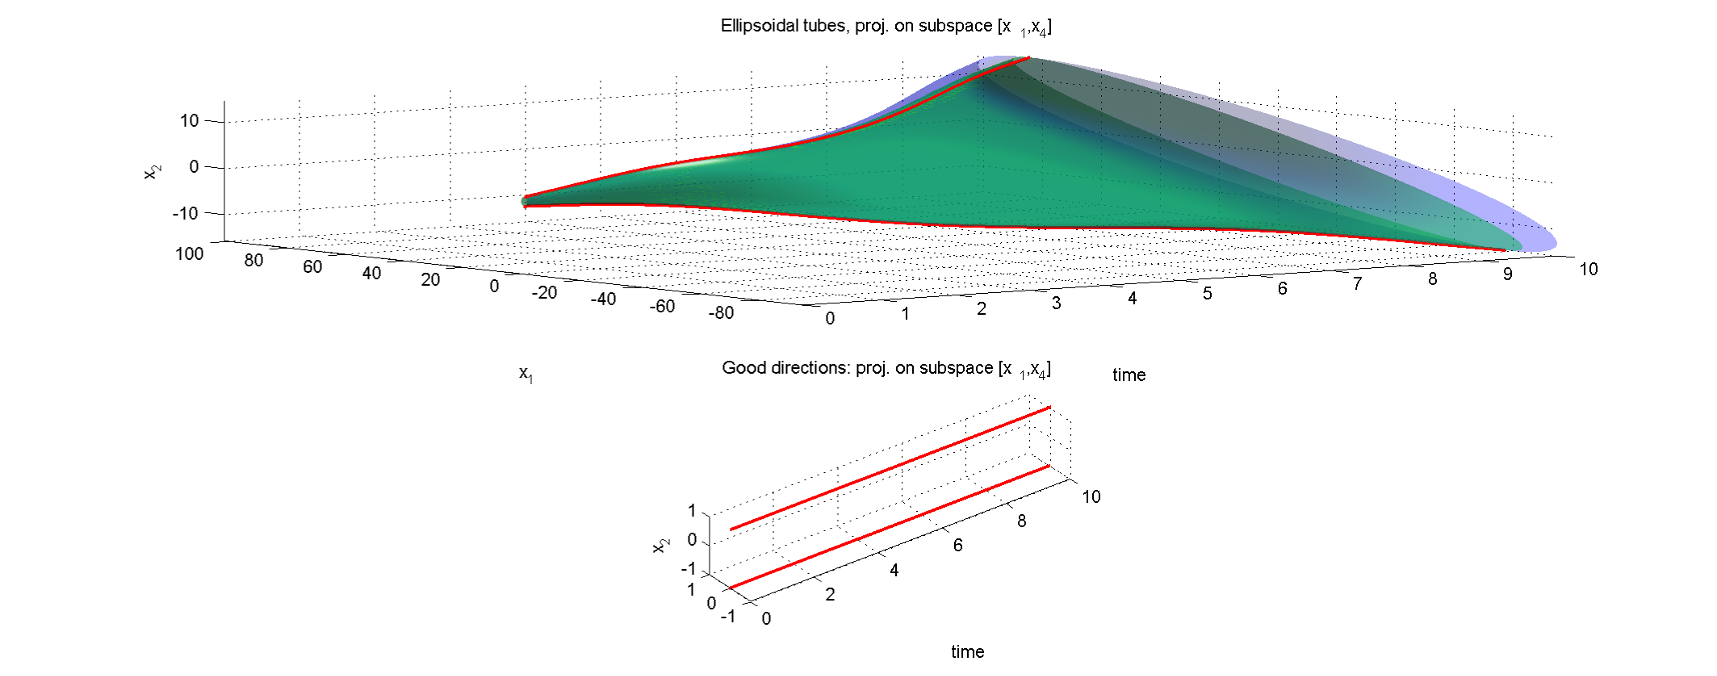
\includegraphics[height=9 cm]{statProj.eps}}
%\caption{Static projection of the ellipsoidal tube.}
%\end{figure}

\easytwofigures{reachTube_dynProj.png}{Static projection of the ellipsoidal tube}{stat_proj}{reachTube_staticProj.png}{Dynamic projection of the ellipsoidal tube.}{dyn_proj}{Projection of the ellipsoidal tube.}{}


%\begin{figure}[htbp]
%\centerline{
%\includegraphics[height=9 cm]{dynProj.eps}}
%\caption{Dynamic projection of the ellipsoidal tube.}
%\label{ellpolyfig}
%\end{figure}
We can compute tubes by the instant of time using method{\tt fromEllTubes}:
\verbmcodef[Computing the tubes by the instant of time]{mcodesnippets/s_chapter05_section03_snippet05.m}
Also we can get initial data from the resulting tube:
\verbmcodef[Getting the initial ellipsoidal array]{mcodesnippets/s_chapter05_section03_snippet06.m}
There is a method to display a content of ellipsoidal tubes.
\verbmcodef[Display a content of the ellipsoidal tube]{mcodesnippets/s_chapter05_section03_snippet07.m}
%\begin{figure}[htbp]
%\centerline{
%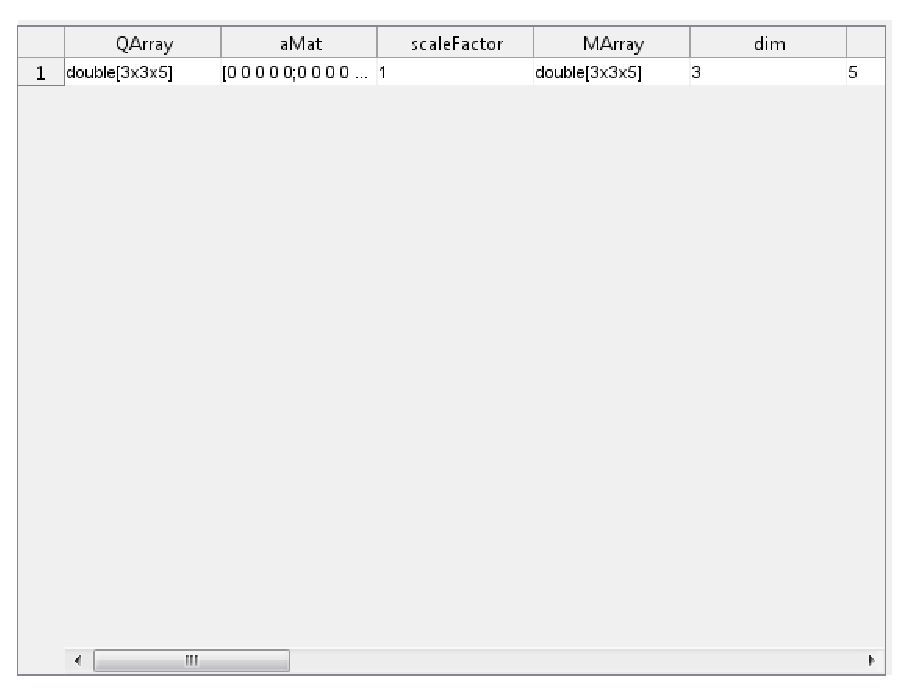
\includegraphics[height=10 cm]{dispPic.eps}}
%\caption{Content of the ellipsoidal tube}
%\end{figure}

\easyfigure{dispPic.eps}{Content of the ellipsoidal tube}{dispPic}

There are several methods to find the tubes with necessary parameters.
\verbmcodef[Filtering of the tube by 'sTime' parameter]{mcodesnippets/s_chapter05_section03_snippet08.m}
Also you can use the method {\tt display} to see the result of the method's work.
\verbmcodef[Selection of the tube by index]{mcodesnippets/s_chapter05_section03_snippet09.m}
We can sort our tubes by certain fields:
\verbmcodef[Sorting of the tubes]{mcodesnippets/s_chapter05_section03_snippet10.m}
\section{Reachability}
To compute the reach sets of the systems described in chapter 3, we define
few new classes in the {\it Ellipsoidal Toolbox}: class {\tt LinSysContinuous}
for the continuous-time system description, class {\tt LinSysDiscrete}
for the discrete-time system description and classes {\tt ReachContinuous$\backslash$ReachDiscrete} for the reach set data. We start by explaining how to define a system
using {\tt LinSysContinuous} object. Also we can use {\tt LinSysFactory} class for the description of this system.
Through it's method {\tt create} user can get {\tt LinSysContinuous} or {\tt LinSysDiscrete} object.
For example, description of the system
\[ \left[\begin{array}{cc}
\dot{x}_1\\
\dot{x}_2\end{array}\right] = \left[\begin{array}{cc}
0 & 1\\
0 & 0\end{array}\right]\left[\begin{array}{c}
x_1\\
x_2\end{array}\right] + \left[\begin{array}{c}
u_1(t)\\
u_2(t)\end{array}\right], ~~~ u(t)\in\EE(p(t), P) \]
with
\[ p(t) = \left[\begin{array}{c}
\sin(t)\\
\cos(t)\end{array}\right], ~~~ P = \left[\begin{array}{cc}
9 & 0\\
0 & 2\end{array}\right], \]
is done by the following sequence of commands:
\verbmcodef[Description of the system]
{mcodesnippets/s_chapter05_section04_snippet01.m}
If matrices $A$ or $B$ depend on time, say $A(t)=\left[\begin{array}{cc}
0 & 1-\cos(2t)\\
-\frac{1}{t} & 0\end{array}\right]$, then matrix {\tt aMat} should be symbolic:
\verbmcodef[A(t) -- time-variant]
{mcodesnippets/s_chapter05_section04_snippet02.m}
To describe the system with disturbance
\[ \left[\begin{array}{cc}
\dot{x}_1\\
\dot{x}_2\end{array}\right] = \left[\begin{array}{cc}
0 & 1\\
0 & 0\end{array}\right]\left[\begin{array}{c}
x_1\\
x_2\end{array}\right] + \left[\begin{array}{c}
u_1(t)\\
u_2(t)\end{array}\right] + \left[\begin{array}{c}
0\\
1\end{array}\right]v(t), \]
with bounds on control as before, and disturbance being $-1\leq v(t)\leq1$,
we type:
\verbmcodef[Description of the system with disturbance]
{mcodesnippets/s_chapter05_section04_snippet03.m}
Control and disturbance bounds {\tt SUBounds} and {\tt vEllObj} can have different types.
If the bound is constant, it should be described by {\tt ellipsoid} object.
If the bound depends on time, then it is represented by a structure with
fields {\tt center} and {\tt shape}, one or both of which are symbolic.
In system {\tt sys}, the control bound {\tt SUBounds} is defined as such a structure.
Finally, if the control or disturbance is known and fixed, it should be
defined as a vector, of type {\tt double} if constant, or symbolic, if
it depends on time.

To declare a discrete-time system
\[ \left[\begin{array}{c}
x_1[k+1]\\
x_2[k+1]\end{array}\right] = \left[\begin{array}{cc}
0 & 1\\
-1 & -0.5\end{array}\right]\left[\begin{array}{c}
x_1[k]\\
x_2[k]\end{array}\right] + \left[\begin{array}{c}
0\\
1\end{array}\right]u[k], ~~~ -1\leq u[k]\leq 1,\]
we use {\tt LinSysDiscrete} constructor:
\verbmcodef[Description of the discrete-time system]
{mcodesnippets/s_chapter05_section04_snippet04.m}
Once the {\tt LinSysDiscrete} object is created, we need to specify the set
of initial conditions, the time interval and values of the direction vector,
for which the reach set approximations must be computed:
\verbmcodef[Description of an initial data]
{mcodesnippets/s_chapter05_section04_snippet05.m}
The reach set approximation is computed by calling the constructor
of the {\tt ReachContinuous} object:
\verbmcodef[Computation of the reach set approximation]
{mcodesnippets/s_chapter05_section04_snippet06.m}
At this point, variable {\tt firstRsObj} contains the reach set approximations for the
specified continuous-time system, time interval and set of initial conditions
computed for given directions. Both external and internal
approximations are computed.
The reach set approximation data can be
extracted in the form of arrays of ellipsoids:
\verbmcodef[Extraction of the reach set approximation data]{mcodesnippets/s_chapter05_section04_snippet07.m}

Ellipsoidal arrays {\tt externallEllMat} and {\tt internalEllMat} have $4$ rows because we computed
the reach set approximations for $4$ directions. Each row of ellipsoids
corresponds to one direction. The number of columns in {\tt externallEllMat} and {\tt internalEllMat}
is defined by the {\tt nTimeGridPoints} parameter, which is available from {\tt elltool.conf.Properties}
static class (see chapter 6 for details). It represents the number of time values
in our time interval, at which the approximations are evaluated. These
time values are returned in the optinal output parameter, array {\tt timeVec},
whose length is the same as the number of columns in {\tt externallEllMat} and {\tt internalEllMat}.
Intersection of ellipsoids in a particular column of {\tt externallEllMat} gives
external ellipsoidal approximation of the reach set at corresponding time.
Internal ellipsoidal approximation of this set at this time is given by the
union of ellipsoids in the same column of {\tt internalEllMat}.

We may be interested in the reachability data of our system in some
particular time interval, smaller than the one for which the reach set was
computed, say $3\leq t\leq5$.
This data can be extracted and returned in the form of {\tt ReachContinuous}
object by the {\tt cut} function:
\verbmcodef[Get the reachability data in the time interval]{mcodesnippets/s_chapter05_section04_snippet08.m}

To obtain a snap shot of the reach set at given time, the same function
{\tt cut} is used:
\verbmcodef[Obtaining of the snap shot at given time]{mcodesnippets/s_chapter05_section04_snippet09.m}
It can be checked if the external or internal reach set approximation
intersects with given ellipsoids, hyperplanes or polytopes:
\verbmcodef[Check if ellipsoid intersects with external approximation]{mcodesnippets/s_chapter05_section04_snippet10.m}
\verbmcodef[Check if ellipsoid intersects with internal approximation]{mcodesnippets/s_chapter05_section04_snippet11.m}
\verbmcodef[Check if hyperplanes intersect with internal approximation]{mcodesnippets/s_chapter05_section04_snippet12.m}
\verbmcodef[Check if polytope intersects with external approximation]{mcodesnippets/s_chapter05_section04_snippet13.m}




If a given set intersects with the internal approximation of the reach set,
then this set intersects with the actual reach set.
If the given set does not
intersect with external approximation, this set does not
intersect the actual reach set. There are situations, however, when the
given set intersects with the external approximation but does not intersect
with the internal one. In our example above, ellipsoid {\tt ellObj} is such a case:
the quality of the approximation does not allow us to determine whether or not
{\tt ellObj} intersects with the actual reach set. To improve the quality
of approximation, {\tt refine} function should be used:
\verbmcodef[Check if the ellipsoid intersects the internal approximation]{mcodesnippets/s_chapter05_section04_snippet14.m}

Now we are sure that ellipsoid {\tt ellObj} intersects with the actual reach set.
%Recall that when we computed reach set {\tt firstRsObj} the first time, we did it
%with the option {\tt save\_all} set to $1$. This option indicated to the
%{\tt reach} constructor that it should save all intermediate calculations of
%data in the {\tt reach} object {\tt firstRsOb}. These data include evaluations
%of matrices $A$, $B$, $G$ at specific time values (in case these
%matrices depend on time) together with the control and disturbance
%bounds, the state transition matrix and its inverse evaluated at
%these time values.
%By default, {\tt save\_all} option is set to $0$, and all these intermediate
%data are not retained, which significantly reduces the memory used
%by the {\tt reach} object {\tt firstRsObj}.
However, to use the {\tt refine} function,
the reach set object must contain all calculated data, otherwise, an
error is returned.

Having a reach set object resulting from the {\tt ReachContinuous}, {\tt cut} or
{\tt refine} operations, we can obtain the trajectory of the center
of the reach set and the good curves along which the actual reach set
is touched by its ellipsoidal approximations:
\verbmcodef[Obtaining the trajectory of the center
of the reach set and the good curves]{mcodesnippets/s_chapter05_section04_snippet15.m}

Variable {\tt ctrMat} here is a matrix whose columns are the points ofthe
reach set center trajectory evaluated at time values returned in the
array {\tt ttVec}. Variable {\tt gcCMat} contains $4$ matrices each of which
corresponds to a good curve (columns of such matrix are points of the
good curve evaluated at time values in {\tt ttVec}).
The analytic expression for the control driving the system along a good
curve is given by formula (\ref{uct}).

We computed the reach set up to time $10$. It is possible to continue
the reach set computation for a longer time horizon using the reach set
data at time $10$ as initial condition.
It is also possible that the dynamics and inputs of the system change at
certain time, and from that point on the system evolves according to the new
system of differential equations. For example, starting at time $10$, our
reach set may evolve in time according to the time-variant system {\tt sys\_t}
defined above. Switched systems are a special case of this situation.
To compute the further evolution in time of the existing reach set,
function {\tt evolve} should be used:
\verbmcodef[Computation of the further evolution in time of the reach set]{mcodesnippets/s_chapter05_section04_snippet16.m}
Function {\tt evolve} can be viewed as an implementation of the semigroup
property.

To compute the backward reach set for some specified target set,
we declare the time interval so that the terminating time comes first:
\verbmcodef[Computation of the backward reach set]{mcodesnippets/s_chapter05_section04_snippet17.m}

Reach set and backward reach set computation for discrete-time systems and
manipulations with the resulting reach set object are performed using
the same functions as for continuous-time systems:
\verbmcodef[Computation of reach set and backward reach set for discrete-time systems]
{mcodesnippets/s_chapter05_section04_snippet18.m}

Number of columns in the ellipsoidal arrays {\tt externalEllMat} and {\tt internalEllMat} is $51$
because the backward reach set is computed for $50$ time steps, and the first
column of these arrays contains $3$ ellipsoids {\tt yEllObj} - the terminating
condition.

When dealing with discrete-time systems, all functions that accept time or
time interval as an input parameter, round the time values and treat them as
integers.
\section{Properties}
\todo[inline]{Added this section}
Functions of the {\it Ellipsoidal Toolbox} can be called with
user-specified values of certain global parameters. System of the parameters
are configured using xml files, which  available from a set of command-line
utilities:
\verbmcodef[Configuration download]
{mcodesnippets/s_chapter05_section05_snippet01.m}
Here we list system parameters available from the 'default' configuration:
\begin{enumerate}
\item {\tt version = '1.4dev'} - current version of {\it ET}.
\item {\tt isVerbose = false} - makes all the calls to {\it ET}
routines silent, and no information except errors is displayed.
\item {\tt absTol = 1e-7} - absolute tolerance.
\item {\tt relTol = 1e-5} - relative tolerance.
\item {\tt nTimeGridPoints = 200} - density of the time grid for the
continuous time reach set computation.
This parameter directly affects the number of ellipsoids to
be stored in the {\tt ReachContinuous$\backslash$ReachDiscrete} object.
\item {\tt ODESolverName = ode45} - specifies the ODE solver for continuous time
reach set computation.
\item {\tt isODENormControl = 'on'} - switches on and off the norm control
in the ODE solver. When turned on, it slows down the computation, but improves
the accuracy.
\item {\tt isEnabledOdeSolverOptions = false} - when set to {\tt false}, calls the ODE solver
without any additional options like norm control. It makes the computation
faster but less accurate. Otherwise, it is assumed to be {\tt true}, and only in this
case the previous option makes a difference.
\item {\tt nPlot2dPoints = 200} - the number of points used to plot a
2D ellipsoid. This parameter also affects the quality of 2D reach tube
and reach set plots.
\item {\tt nPlot3dPoints = 200} - the number of points used to plot
a 3D ellipsoid. This parameter also affects the quality of 3D reach set plots.
\end{enumerate}
Once the configuration is loaded, the system parameters are available through
{\tt elltool.conf.Properties}.
{\tt elltool.conf.Properties} is a static class, providing emulation of static
properties for toolbox. It has two function types: setters and getters.
Using getters we obtain system parameters.
\verbmcodef[Getting parameters]
{mcodesnippets/s_chapter05_section05_snippet02.m}
 Some of the parameters can be changed
in run-time via setters.
\verbmcodef[Changing parameters]
{mcodesnippets/s_chapter05_section05_snippet03.m}
\section{Visualization}
{\it Ellipsoidal Toolbox} has several plotting routines:
\begin{itemize}
\item {\tt ellipsoid/plot} - plots one or more ellipsoids, or arrays of
ellipsoids, defined in ${\bf R}$, ${\bf R}^2$ or ${\bf R}^3$.
\item {\tt ellipsoid/minksum} - plots geometric sum of finite number of
ellipsoids defined in ${\bf R}$, ${\bf R}^2$ or ${\bf R}^3$.
\item {\tt ellipsoid/minkdiff} - plots geometric difference
(if it is not an empty set) of two ellipsoids defined in
${\bf R}$, ${\bf R}^2$ or ${\bf R}^3$.
\item {\tt ellipsoid/minkmp} - plots geometric (Minkowski) sum
of the geometric difference of two ellipsoids and the geometric sum of $n$
ellipsoids defined in ${\bf R}$, ${\bf R}^2$ or ${\bf R}^3$.
\item {\tt ellipsoid/minkpm} - plots geometric (Minkowski) difference of the
geometric sum of ellipsoids and a single ellipsoid defined in
${\bf R}$, ${\bf R}^2$ or ${\bf R}^3$.
\item {\tt hyperplane/plot} - plots one or more hyperplanes, or arrays of
hyperplanes, defined in ${\bf R}^2$ or ${\bf R}^3$.
\item {\tt reach/plot\_ea} - plots external approximation of the reach set
whose dimension is $2$ or $3$.
\item {\tt reach/plot\_ia} - plots internal approximation of the reach set
whose dimension is $2$ or $3$.
\end{itemize}
All these functions allow the user to specify the color of the plotted objects,
line width for 1D and 2D plots, and transparency level of the 3D objects.
Hyperplanes are displayed as line segments in 2D and square facets in 3D.
In the {\tt hyperplane/plot} method it is possible to specify the center
of the line segment or facet and its size.

Ellipsoids of dimensions higher than three must be
projected onto a two- or three-dimensional subspace before being plotted.
This is done by means of {\tt projection} function:
\verbmcodef[Projection of the ellipsoids onto a two- or three-dimensional subspace]
{mcodesnippets/s_chapter05_section06_snippet01.m}

Since the operation of projection is linear, the projection of the geometric
sum of ellipsoids equals the geometric sum of the projected ellipsoids.
The same is true for the geometric difference of two ellipsoids.

Function {\tt projection} exists also for the {\tt ReachContinuous$\backslash$ReachDiscrete} objects:
\verbmcodef[Projection of the reach set tube]
{mcodesnippets/s_chapter05_section06_snippet02.m}

The quality of the ellipsoid and reach set plots is controlled by the
parameters {\tt nPlot2dPoints} and {\tt nPlot3dPoints}, which are available
from getters of ellipsoid class.

